\documentclass[conference]{IEEEtran}
\usepackage{amsmath,amssymb}
\usepackage{booktabs}
\usepackage{array}
\usepackage{multirow}
\usepackage{xcolor}
\usepackage{tikz}
\usetikzlibrary{arrows.meta,positioning,calc,fit,backgrounds}
\usepackage{pgfplots}
\pgfplotsset{compat=1.18}
\usepackage{newtxtext,newtxmath}
\usepackage{url}
\usepackage{microtype}
\usepackage{enumitem}
\usepackage{float}
\usepackage{needspace}
\setlist[itemize]{leftmargin=*,nosep}

\definecolor{cblue}{HTML}{2D6F9F}
\definecolor{corange}{HTML}{D97728}
\definecolor{cgreen}{HTML}{2E7D62}
\definecolor{cred}{HTML}{A33A32}
\definecolor{cgray}{HTML}{68737D}
\definecolor{clight}{HTML}{EEF2F4}
\definecolor{clightblue}{HTML}{E6F0F6}
\definecolor{clightgreen}{HTML}{E8F3EE}
\definecolor{clightred}{HTML}{F7E9E7}
\definecolor{clightorange}{HTML}{F8EFE5}

\newcommand{\copycat}{\textsc{CopyCAT}}
\newcommand{\rootcopy}{\mathcal{S}}
\newcommand{\tight}{\vspace{-0.7ex}}

\title{\copycat: Visual Certificate Atlas and Reproducibility Supplement}
\author{\IEEEauthorblockN{Sushanth Dasari}
\IEEEauthorblockA{Amity International School, Sector-46, Gurugram, India\\
Supplementary material for the CopyCAT research manuscript}}

\begin{document}
\maketitle

\begin{abstract}
This supplement is a visual, certificate-first companion to the main \copycat{} manuscript. It deliberately follows a simple progression: first show the phenomenon with no abstraction, then derive the exact pairwise certificate, then explain why one leaderboard winner requires a \emph{shared} schedule rather than separate pairwise witnesses, and finally connect every headline claim to an executable check in the public repository. No new scientific claim is introduced here. The purpose is to make the existing finite-archive result easier to audit: on the pinned 588-question MMLU-ProX-Lite archive, GPT needs exactly three shared copies to become uniquely first, Claude needs exactly eight, and seven other configurations are provably excluded under the one-extra-copy-per-root intervention. The same audit distinguishes targeted attainability from random frequency and motivates a mass-preserving repair once trusted root lineage is given.
\end{abstract}

\section{Start With the Smallest Possible Story}
A benchmark score is an average over units that are intended to count once. \copycat{} asks a deliberately narrow question: if the predictions and labels are frozen, but some \emph{existing} units are allowed to count twice, which decisions can change? The same copied-root set must be used for every system. Nothing about the models changes; only what the evaluator counts changes.

\begin{figure}[H]
\centering
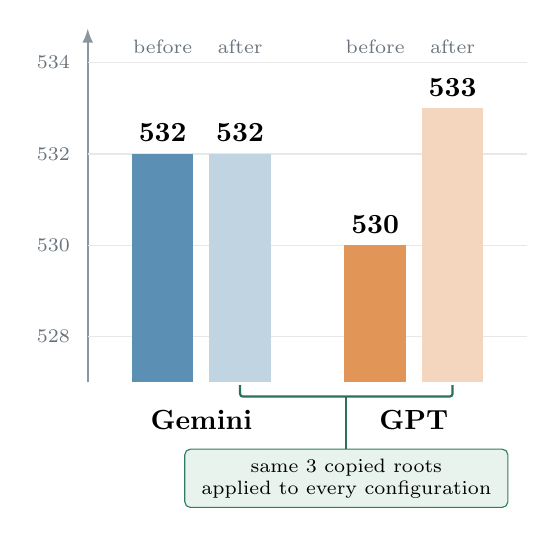
\begin{tikzpicture}[x=0.78cm,y=0.58cm,font=\footnotesize,>=Latex]
  \draw[-{Latex[length=1.8mm]},cgray!75,line width=0.55pt] (0,0) -- (0,7.75);
  \foreach \y/\lab in {1/528,3/530,5/532,7/534}{
    \draw[gray!18,line width=0.45pt] (0,\y) -- (7.15,\y);
    \node[anchor=east,text=cgray,font=\scriptsize] at (-0.13,\y) {\lab};
  }
  \fill[cblue!78]   (0.72,0) rectangle (1.72,5.00);
  \fill[cblue!30]   (1.98,0) rectangle (2.98,5.00);
  \fill[corange!78] (4.18,0) rectangle (5.18,3.00);
  \fill[corange!30] (5.44,0) rectangle (6.44,6.00);
  \node[anchor=south,font=\bfseries] at (1.22,5.05) {532};
  \node[anchor=south,font=\bfseries] at (2.48,5.05) {532};
  \node[anchor=south,font=\bfseries] at (4.68,3.05) {530};
  \node[anchor=south,font=\bfseries] at (5.94,6.05) {533};
  \node[text=cgray,font=\scriptsize] at (1.22,7.35) {before};
  \node[text=cgray,font=\scriptsize] at (2.48,7.35) {after};
  \node[text=cgray,font=\scriptsize] at (4.68,7.35) {before};
  \node[text=cgray,font=\scriptsize] at (5.94,7.35) {after};
  \node[font=\bfseries] at (1.85,-0.82) {Gemini};
  \node[font=\bfseries] at (5.31,-0.82) {GPT};

  % shared-schedule bracket with deliberate breathing room below labels
  \draw[cgreen!90!black,line width=0.8pt,rounded corners=1pt]
        (2.48,-0.06) -- (2.48,-0.31) -- (5.94,-0.31) -- (5.94,-0.06);
  \coordinate (railmid) at (4.21,-0.31);
  \node[draw=cgreen,fill=clightgreen,rounded corners=2pt,align=center,
        inner xsep=6pt,inner ysep=3.4pt,font=\scriptsize] (shared) at (4.21,-2.10)
        {same 3 copied roots\\applied to every configuration};
  \draw[cgreen!90!black,line width=0.8pt] (railmid) -- ++(0,-0.38) -- (shared.north);
\end{tikzpicture}
\caption{The whole headline result before any notation. The outputs and labels are unchanged. Three already-scored roots are counted twice under one common schedule, moving GPT from 530 to 533 correct while Gemini remains at 532.}
\label{fig:headline}
\end{figure}

The lower bound is already visible in Fig.~\ref{fig:headline}. GPT begins two correct answers behind Gemini. A single copied binary root can improve the GPT-minus-Gemini count gap by at most one. A strict win therefore needs at least three favorable copies. The artifact supplies three such roots, so the lower bound is attained.

\section{Now Generalize the Toy Argument}
For a pair of systems $A,B$, let $d_i=z_i^A-z_i^B$ be the fixed score difference on root $i$ and let $D=\sum_i d_i$. If $S$ is the set of copied roots, the new margin is
\begin{equation}
M_{A,B}(S)=\frac{D+\sum_{i\in S}d_i}{n+|S|}.
\label{eq:margin}
\end{equation}
There is no combinatorial mystery in the pairwise case. At exactly $k$ copies, the smallest margin is obtained by copying the $k$ smallest $d_i$ values and the largest margin by copying the $k$ largest values:
\begin{equation}
L_k=\frac{D+\sum_{r=1}^{k}d_{(r)}}{n+k},\qquad
U_k=\frac{D+\sum_{r=n-k+1}^{n}d_{(r)}}{n+k}.
\label{eq:extrema}
\end{equation}
Sorting once therefore gives every exact pairwise budget in $O(n\log n+B)$ time. This sorting principle is established prior work; \copycat{} uses it as one component of a larger shared-schedule audit \cite{alzhrani}.

\begin{figure}[H]
\centering
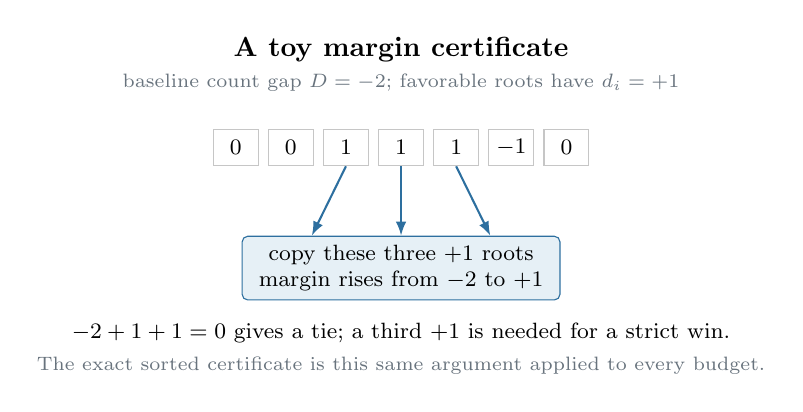
\begin{tikzpicture}[font=\footnotesize,>=Latex]
  \node[font=\bfseries] at (0,0) {A toy margin certificate};
  \node[text=cgray,font=\scriptsize] at (0,-0.43)
        {baseline count gap $D=-2$; favorable roots have $d_i=+1$};
  \foreach \x/\v in {-3/0,-2/0,-1/1,0/1,1/1,2/-1,3/0}{
    \node[draw=gray!45,fill=white,minimum width=0.57cm,minimum height=0.46cm,
          inner sep=0pt] (r\x) at (0.70*\x,-1.25) {$\v$};
  }
  \node[draw=cblue,fill=clightblue,rounded corners=2pt,align=center,
        inner xsep=6pt,inner ysep=3.2pt,minimum width=2.75cm] (pick) at (0,-2.78)
        {copy these three $+1$ roots\\margin rises from $-2$ to $+1$};
  \coordinate (p1) at ($(pick.north west)!0.22!(pick.north east)$);
  \coordinate (p2) at ($(pick.north west)!0.50!(pick.north east)$);
  \coordinate (p3) at ($(pick.north west)!0.78!(pick.north east)$);
  \draw[-{Latex[length=1.8mm]},cblue,line width=0.75pt] (r-1.south) -- (p1);
  \draw[-{Latex[length=1.8mm]},cblue,line width=0.75pt] (r0.south) -- (p2);
  \draw[-{Latex[length=1.8mm]},cblue,line width=0.75pt] (r1.south) -- (p3);
  \node at (0,-3.60) {$-2+1+1=0$ gives a tie; a third $+1$ is needed for a strict win.};
  \node[text=cgray,font=\scriptsize] at (0,-4.02)
        {The exact sorted certificate is this same argument applied to every budget.};
\end{tikzpicture}
\caption{The Feynman version of Eq.~\eqref{eq:extrema}: a copy adds one already-observed per-root difference. Sort those differences, then add the most favorable ones first.}
\label{fig:toy}
\end{figure}

\Needspace{0.42\textheight}
\section{The Hard Part: One Winner Needs One Schedule}
Pairwise reversibility is not enough for a leaderboard claim. A target can beat rival $A$ using one copied-root set and rival $B$ using another, with no single set beating both. This is the key distinction between ``a pair can flip'' and ``this system can actually become the winner.''

\begin{figure}[H]
\centering
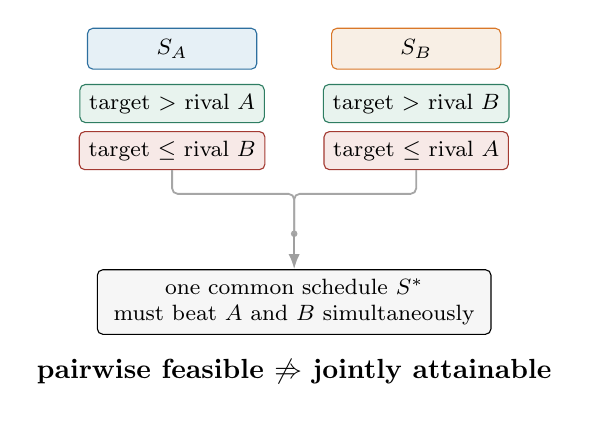
\begin{tikzpicture}[font=\footnotesize,>=Latex]
  \node[draw=cblue,fill=clightblue,rounded corners=2pt,minimum width=2.15cm,
        minimum height=0.52cm] (sa) at (-1.55,0) {$S_A$};
  \node[below=1.8mm of sa,draw=cgreen,fill=clightgreen,rounded corners=2pt,
        minimum width=2.15cm] (aa) {target $>$ rival $A$};
  \node[below=1.0mm of aa,draw=cred,fill=clightred,rounded corners=2pt,
        minimum width=2.15cm] (ab) {target $\le$ rival $B$};
  \node[draw=corange,fill=clightorange,rounded corners=2pt,minimum width=2.15cm,
        minimum height=0.52cm] (sb) at (1.55,0) {$S_B$};
  \node[below=1.8mm of sb,draw=cgreen,fill=clightgreen,rounded corners=2pt,
        minimum width=2.15cm] (bb) {target $>$ rival $B$};
  \node[below=1.0mm of bb,draw=cred,fill=clightred,rounded corners=2pt,
        minimum width=2.15cm] (ba) {target $\le$ rival $A$};
  \coordinate (merge) at (0,-2.35);
  \draw[gray!70,line width=0.65pt,rounded corners=2pt]
        (ab.south) -- ++(0,-3mm) -| (merge);
  \draw[gray!70,line width=0.65pt,rounded corners=2pt]
        (ba.south) -- ++(0,-3mm) -| (merge);
  \fill[gray!70] (merge) circle (1.2pt);
  \node[below=4.5mm of merge,draw=black,fill=gray!7,rounded corners=2pt,
        align=center,minimum width=5.0cm,minimum height=0.78cm] (joint)
        {one common schedule $S^*$\\must beat $A$ and $B$ simultaneously};
  \draw[-{Latex[length=1.9mm]},gray!75,line width=0.75pt] (merge) -- (joint.north);
  \node[below=1.8mm of joint,font=\bfseries] {pairwise feasible $\not\Rightarrow$ jointly attainable};
\end{tikzpicture}
\caption{Why \copycat{} needs a joint winner certificate. Separate pairwise witnesses may be mutually incompatible.}
\label{fig:joint}
\end{figure}

For binary accuracy, roots can be compressed by their outcome pattern $p$ across systems. Let $N_p$ be the number of roots with pattern $p$, $x_p$ the number copied, $C_t$ the target's original correct count, and $a_{t,p}$ the target's bit on pattern $p$. A target $t$ is a unique winner only if the \emph{same} integer vector $x$ satisfies
\begin{equation}
\sum_p x_p(a_{t,p}-a_{j,p})\ge 1-(C_t-C_j),\quad \forall j\ne t,
\label{eq:joint}
\end{equation}
with $0\le x_p\le N_p$, $x_p\in\mathbb Z$, and $\sum_p x_p\le B$. Feasible witnesses are recomputed with integer arithmetic; tiny instances are independently brute-forced.

\Needspace{0.62\textheight}
\section{Certificate Atlas on the Pinned MMLU Archive}
The most useful way to read the ten-system result is not as a leaderboard but as a map of what the allowed intervention can and cannot reach. Figure~\ref{fig:atlas} shows the original counts and the exact winner certificate for every configuration.

\begin{figure}[H]
\centering
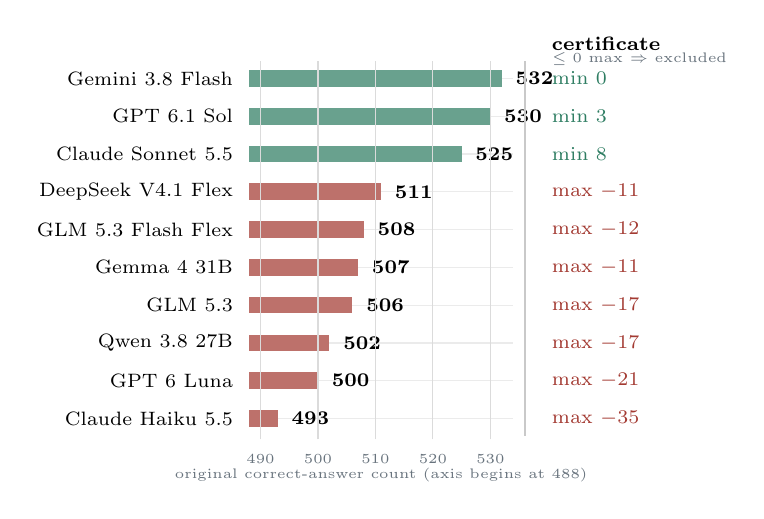
\begin{tikzpicture}[x=0.073cm,y=0.48cm,font=\scriptsize]
  \def\xzero{488}
  \newcommand{\atlasrow}[5]{%
    \node[anchor=east,font=\scriptsize] at (-1.1,#1) {#2};
    \draw[gray!16] (0,#1) -- (46,#1);
    \pgfmathsetmacro{\len}{#3-\xzero}
    \fill[#5!72] (0,#1-0.22) rectangle (\len,#1+0.22);
    \node[anchor=west,font=\bfseries\scriptsize] at (\len+0.7,#1) {#3};
    \node[anchor=west,text=#5,font=\scriptsize,align=left,text width=1.55cm] at (51,#1) {#4};
  }
  \atlasrow{9}{Gemini 3.8 Flash}{532}{min 0}{cgreen}
  \atlasrow{8}{GPT 6.1 Sol}{530}{min 3}{cgreen}
  \atlasrow{7}{Claude Sonnet 5.5}{525}{min 8}{cgreen}
  \atlasrow{6}{DeepSeek V4.1 Flex}{511}{max $-11$}{cred}
  \atlasrow{5}{GLM 5.3 Flash Flex}{508}{max $-12$}{cred}
  \atlasrow{4}{Gemma 4 31B}{507}{max $-11$}{cred}
  \atlasrow{3}{GLM 5.3}{506}{max $-17$}{cred}
  \atlasrow{2}{Qwen 3.8 27B}{502}{max $-17$}{cred}
  \atlasrow{1}{GPT 6 Luna}{500}{max $-21$}{cred}
  \atlasrow{0}{Claude Haiku 5.5}{493}{max $-35$}{cred}
  \foreach \x/\lab in {2/490,12/500,22/510,32/520,42/530}{
    \draw[gray!28] (\x,-0.55) -- (\x,9.45);
    \node[anchor=north,text=cgray,font=\tiny] at (\x,-0.70) {\lab};
  }
  \draw[gray!42,line width=0.5pt] (48,-0.45) -- (48,9.45);
  \node[anchor=north,font=\tiny,text=cgray] at (23,-1.05) {original correct-answer count (axis begins at 488)};
  \node[anchor=west,font=\bfseries\scriptsize] at (51,9.92) {certificate};
  \node[anchor=west,font=\tiny,text=cgray] at (51,9.52) {$\le 0$ max $\Rightarrow$ excluded};
\end{tikzpicture}
\caption{Complete winner atlas for the pinned 588-root MMLU-ProX-Lite archive. Exactly three configurations are attainable unique winners under the allowed one-extra-copy-per-root intervention. GPT needs exactly 3 copies, Claude exactly 8, and the other seven receive solver-independent blocking-rival exclusions. ``Max'' is the best possible target-minus-Gemini correct-count advantage after copying every root favorable to that target; a nonpositive value excludes a unique win.}
\label{fig:atlas}
\end{figure}

The three-copy GPT witness uses root indices $\{277,507,424\}$ and yields final correct counts $533$ for GPT and $532$ for Gemini. The eight-copy Claude witness uses $\{322,380,190,424,393,245,15,564\}$ and yields Claude $533$, Gemini $532$, GPT $531$. These are not merely solver outputs: the initial deficits imply the lower bounds of three and eight, and the supplied schedules attain them.

\Needspace{0.38\textheight}
\section{Attainability Is Not Frequency}
A targeted certificate answers ``can this happen under the declared rule?'' A random control answers ``how often does it happen under one specific randomization?'' Those are different questions.

\begin{figure}[H]
\centering
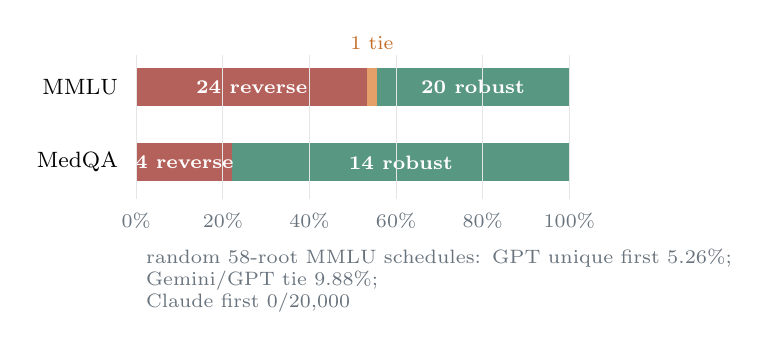
\begin{tikzpicture}[font=\footnotesize,x=0.055cm,y=0.8cm]
  % MMLU stacked bar
  \node[anchor=east] at (-2,2.5) {MMLU};
  \fill[cred!80] (0,2.2) rectangle (53.3,2.8);
  \fill[corange!70] (53.3,2.2) rectangle (55.5,2.8);
  \fill[cgreen!80] (55.5,2.2) rectangle (100,2.8);
  \node[text=white,font=\bfseries\scriptsize] at (26.65,2.5) {24 reverse};
  \node[text=white,font=\bfseries\scriptsize] at (77.75,2.5) {20 robust};
  \node[font=\scriptsize,anchor=south,text=corange!90!black] at (54.4,2.93) {1 tie};
  % MedQA
  \node[anchor=east] at (-2,1.3) {MedQA};
  \fill[cred!80] (0,1.0) rectangle (22.2,1.6);
  \fill[cgreen!80] (22.2,1.0) rectangle (100,1.6);
  \node[text=white,font=\bfseries\scriptsize] at (11.1,1.3) {4 reverse};
  \node[text=white,font=\bfseries\scriptsize] at (61.1,1.3) {14 robust};
  \foreach \x in {0,20,40,60,80,100}{\draw[gray!20] (\x,0.72) -- (\x,3.0);\node[anchor=north,text=cgray,font=\scriptsize] at (\x,0.65) {\x\%};}
  \node[anchor=north west,text=cgray,font=\scriptsize,align=left,text width=7.4cm] at (0,0.08) {random 58-root MMLU schedules: GPT unique first 5.26\%; Gemini/GPT tie 9.88\%;\\Claude first 0/20,000};
\end{tikzpicture}
\caption{Decision classes at the 10\% copy budget. MMLU contains many targeted reversals; MedQA is mostly robust. Random schedules are a frequency diagnostic, not a replacement for attainability certificates.}
\label{fig:robust}
\end{figure}

For MMLU at $B=58$, 24 of 45 strict pooled orders can reverse, one is tie-only, and 20 are strictly robust. Yet among 20,000 label-blind random 58-root schedules, GPT is uniquely first only 1,051 times (5.26\%), 1,975 produce a Gemini/GPT tie, and Claude is never first. MedQA gives a different profile: four of 18 Brier comparisons reverse within $B=127$ and 14 remain robust; the minimum reversal budgets are 71, 77, 100, and 105 roots.

\Needspace{0.42\textheight}
\section{What the Repair Fixes -- and What It Does Not}
If trusted lineage says several descendants are only alternate representations of one unchanged root, they should split that root's mass rather than create extra mass. If descendant masses $v_{ij}$ satisfy $\sum_j v_{ij}=w_i$, then for an unchanged root value $z_i$,
\begin{equation}
\sum_j v_{ij}z_i = w_i z_i.
\label{eq:mass}
\end{equation}

\begin{figure}[H]
\centering
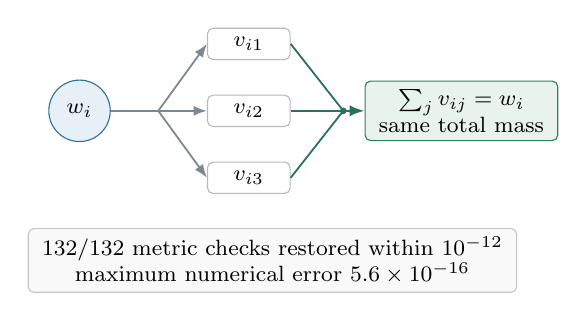
\begin{tikzpicture}[font=\footnotesize,>=Latex]
  \node[draw=cblue,fill=clightblue,circle,minimum size=0.78cm] (root) at (0,1.35) {$w_i$};
  \coordinate (split) at (1.00,1.35);
  \draw[cgray!85,line width=0.7pt] (root.east) -- (split);
  \node[draw=gray!55,fill=white,rounded corners=2pt,minimum width=1.05cm] (a) at (2.15,2.20) {$v_{i1}$};
  \node[draw=gray!55,fill=white,rounded corners=2pt,minimum width=1.05cm] (b) at (2.15,1.35) {$v_{i2}$};
  \node[draw=gray!55,fill=white,rounded corners=2pt,minimum width=1.05cm] (c) at (2.15,0.50) {$v_{i3}$};
  \draw[-{Latex[length=1.7mm]},cgray!85,line width=0.65pt] (split) -- (a.west);
  \draw[-{Latex[length=1.7mm]},cgray!85,line width=0.65pt] (split) -- (b.west);
  \draw[-{Latex[length=1.7mm]},cgray!85,line width=0.65pt] (split) -- (c.west);
  \coordinate (merge) at (3.35,1.35);
  \draw[cgreen!90!black,line width=0.65pt] (a.east) -- (merge);
  \draw[cgreen!90!black,line width=0.65pt] (b.east) -- (merge);
  \draw[cgreen!90!black,line width=0.65pt] (c.east) -- (merge);
  \fill[cgreen!90!black] (merge) circle (1.2pt);
  \node[draw=cgreen,fill=clightgreen,rounded corners=2pt,align=center,
        inner xsep=5pt,inner ysep=3pt,minimum width=2.25cm] (ok) at (4.85,1.35)
        {$\sum_j v_{ij}=w_i$\\same total mass};
  \draw[-{Latex[length=1.9mm]},cgreen!90!black,line width=0.8pt] (merge) -- (ok.west);
  \node[draw=gray!45,fill=gray!5,rounded corners=2pt,align=center,
        inner xsep=5pt,inner ysep=3pt,minimum width=5.25cm] at (2.45,-0.55)
        {132/132 metric checks restored within $10^{-12}$\\maximum numerical error $5.6\times10^{-16}$};
\end{tikzpicture}
\caption{Mass preservation removes multiplicity that is purely representational. It does not discover semantic equivalence; trusted lineage remains an input.}
\label{fig:mass}
\end{figure}

The negative controls matter as much as the positive witnesses. Literal normalized-string deduplication reverses no FActScore model pair. Observed human/model fact-count transport shifts the response-macro aggregate by $+1.03$ points but reverses no matched-topic model order. A large FaStFact coarsening effect is explained by the scoring identity itself. These failures prevent a much stronger but unsupported claim that natural semantic duplication is already common.

\Needspace{0.42\textheight}
\section{Reproducibility Ladder}
The public repository exposes a short reproduction path from the headline result to the full audit without model inference or paid APIs. Figure~\ref{fig:repro} shows that path.

\begin{figure}[H]
\centering
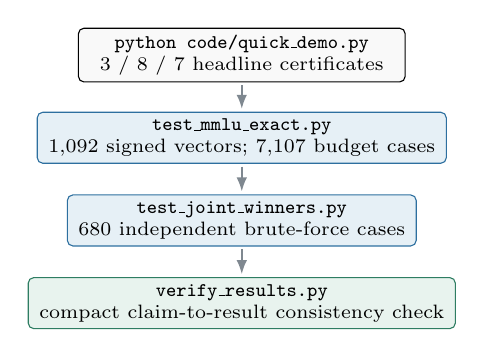
\begin{tikzpicture}[font=\scriptsize,>=Latex]
  \tikzset{flowbox/.style={rounded corners=2pt,minimum width=4.15cm,minimum height=0.63cm,align=center,inner xsep=4pt,inner ysep=2.4pt}}
  \node[flowbox,draw=black,fill=gray!5] (r1) at (0,0)
        {\texttt{python code/quick\_demo.py}\\3 / 8 / 7 headline certificates};
  \node[flowbox,draw=cblue,fill=clightblue] (r2) at (0,-1.05)
        {\texttt{test\_mmlu\_exact.py}\\1,092 signed vectors; 7,107 budget cases};
  \node[flowbox,draw=cblue,fill=clightblue] (r3) at (0,-2.10)
        {\texttt{test\_joint\_winners.py}\\680 independent brute-force cases};
  \node[flowbox,draw=cgreen,fill=clightgreen] (r4) at (0,-3.15)
        {\texttt{verify\_results.py}\\compact claim-to-result consistency check};
  \foreach \u/\v in {r1/r2,r2/r3,r3/r4}{
    \draw[-{Latex[length=1.8mm]},cgray!85,line width=0.75pt,shorten <=1pt,shorten >=1pt]
          (\u.south) -- (\v.north);
  }
\end{tikzpicture}
\caption{Reproduction path for the headline and independent regression checks. The reproduction record also includes a 51-check manuscript quantitative audit, verification of all 140 English MMLU files, and 5,880 raw score rows.}
\label{fig:repro}
\end{figure}

\begin{table}[H]
\caption{Claim-to-artifact map}
\label{tab:map}
\centering
\footnotesize
\begin{tabular}{p{0.31\columnwidth}p{0.61\columnwidth}}
\toprule
Claim & Reproduction artifact \\
\midrule
3-copy GPT minimum & \texttt{headline\_certificate.json} + \texttt{reproduce\_headline.py} \\
8-copy Claude minimum & same certificate + integer deficit lower bound \\
7 impossible winners & blocking-rival fields in \texttt{headline\_certificate.json} \\
24/1/20 pooled classes & \texttt{pooled\_summary.json} \\
MedQA / repair / factuality & \texttt{secondary\_summary.json} \\
Independent regression record & \texttt{reproduction\_checks.json} \\
\bottomrule
\end{tabular}
\end{table}

\section{Scope Boundary in One Sentence}
\copycat{} certifies what a \emph{declared bounded copy intervention} can change in a fixed released archive. It does not estimate how often semantic duplication occurs naturally, discover canonical roots, or establish population-level model superiority. The useful output is therefore not ``this leaderboard is wrong,'' but a more operational statement: \emph{under this evaluator transformation, these winner changes are attainable, these minima are exact, and these other winners are impossible.}

\section*{Code and Data}
Public repository: \url{https://github.com/sushxnthd/copyCAT}. The repository contains the compact lossless 588$\times$10 headline matrix, attained witnesses, exact exclusions, pinned source acquisition, integrity checks, pairwise and joint-winner code, independent tests, secondary summaries, provenance, and a fresh verification record. No model inference or API key is required for the headline checks.

{\scriptsize
\begin{thebibliography}{2}
\bibitem{main} S. Dasari, ``CopyCAT: Exact Winner Certificates When One Fact Counts Twice,'' research manuscript, Nov. 2026.
\bibitem{alzhrani} K. M. Alzhrani, ``Decision Reliability Profiles for Auditing Targeted Case-Removal Sensitivity in AI Model Comparisons Under Additive Metrics,'' \emph{Algorithms}, vol. 19, no. 8, p. 676, 2026.
\end{thebibliography}
}

\end{document}
